\documentclass[11pt]{article}

\usepackage[utf8]{inputenc}
\usepackage[T1]{fontenc}
\usepackage{lmodern}
\usepackage[margin=1in]{geometry}
\usepackage{amsmath}
\usepackage{booktabs}
\usepackage{tabularx}
\usepackage{graphicx}
\usepackage{enumitem}
\usepackage{xcolor}
\usepackage[authoryear,round]{natbib}
\usepackage[colorlinks=true,linkcolor=blue!50!black,citecolor=blue!50!black,urlcolor=blue!50!black]{hyperref}


\title{When the Backtest Lies: Lessons from a Spent Single-Use Holdout\\
and an Open-Source Toolkit for Validating Systematic Strategies}

\author{Joaqu\'in Dom\'inguez\thanks{Independent researcher; MSc in Finance, Universidade de Vigo. Corresponding author: \texttt{joaquindom.p@gmail.com}.} \and Mateo Dom\'inguez\thanks{Independent researcher.}}

\date{Working paper --- draft of 27 October 2026}

\begin{document}
\maketitle

\begin{abstract}
\noindent
We report, with full disclosure of what went wrong, the validation history of LockIn, a long-only quality and trend strategy on the S\&P~500 wrapped in a multi-agent large-language-model (LLM) narrative layer. The project followed a textbook protocol: a train/validation/test split, frozen and pre-registered configurations, an append-only protocol log, and a software guard that allows the 2022--2024 test window to be run exactly once. The pre-registered primary arm earned 12.6\% a year with a Sharpe ratio of 1.47 in sample (2010--2021) and $-2.0\%$ a year with a Sharpe ratio of $-0.53$ on the holdout, against $+10.1\%$ for SPY. We reproduced the holdout exactly three months later and then found that the database it ran on was not fit for purpose: about 21\% of index members had no current fundamentals in 2023--2024, even though the internal data preflight had passed. The one-shot test had been spent on uncertified data. A diagnostic rerun on a later, corrected database moved the result by only $+0.06$ percentage points a year, so the data hole did not cause the failure. That conclusion, however, was only available by looking again at a window that was already spent. The same failure mode then recurred in a second single-use window (1999--2008), through incomplete input fields rather than missing rows. An attribution of the 11.8\,pp a year gap to SPY (on the engine's execution grid) assigns about 41\% to a long-duration Treasury sleeve during a rate shock, 28\% to the cap-weighted benchmark, and 30\% to the equity sleeve, whose selection effect is statistically indistinguishable from zero. We distil the episode into a checklist and introduce \texttt{lockin-validate}, an open-source, offline toolkit whose checks map onto the failure modes we met. Its design rules are that every finding links to evidence, no check reports a pass it could not verify, originals are read-only, and expected outcomes come from an oracle independent of the code under test. Version 0.3.0 widens the toolkit beyond backtests with six use-case modules (alpha signals, supervised models, VaR and ES backtests, point forecasts, portfolio weights and live track records), evaluated on 57 further synthetic cases and two pre-registered adversarial reviews. We make no claim of profitability, certification or regulatory compliance.
\end{abstract}

\medskip
\noindent\textbf{Keywords:} backtest overfitting; holdout; pre-registration; point-in-time data; data certification; look-ahead bias; large language models; model validation; performance attribution.

\noindent\textbf{JEL:} G11, G17, C52, C80.

\section{Introduction}

A backtest is a claim about the past made by someone who already knows how the past ended. The literature has spent two decades cataloguing how that knowledge leaks into results. Multiple testing inflates the best Sharpe ratio among many trials \citep{BaileyEtAl2014Notices,BaileyLopezDePrado2014,HarveyLiuZhu2016}. Published anomalies decay once they leave the sample and once they are published \citep{McLeanPontiff2016}, and many do not survive basic controls \citep{HouXueZhang2020}. Survivorship and look-ahead in the data quietly favour the strategy \citep{BrownEtAl1992}. Large language models (LLMs) add a new channel: a model trained after the test period may simply remember what happened \citep{GlassermanLin2023,LopezLiraTangZhu2025,LiEtAl2025ProfitMirage}.

The standard defence is a protocol: separate training from validation, pre-register the configuration, and touch a final test set once \citep{ArnottHarveyMarkowitz2019,LopezDePrado2018}. This paper is a case study of what happens when a small team actually follows that protocol, and of the ways it can still fail. We are the authors of LockIn, a system that began as the first author's MSc thesis \citep{Dominguez2026TFM}. In July 2026 we spent our single-use 2022--2024 holdout on three pre-registered arms. All three lost money while SPY gained about 10\% a year. Three months later, an independent data audit found that the database used for that run was missing current fundamentals for about a fifth of the universe in 2023--2024. Our internal preflight checks had passed it.

We think the episode is useful to others for three reasons. First, it is a documented negative result. Every look at the validation window, every reproduction and every data correction is logged with dates, and nothing was re-tuned on the test window. Second, it isolates a failure mode that protocol papers mention but rarely dramatise. The holdout is a scarce, non-renewable resource. Spending it before the data are certified wastes it, whether or not the data defect turns out to matter. In our case it did not matter, but we could only learn that by looking again at a spent window. The failure then recurred in a second single-use window through a different mechanism. Third, the post-mortem forced us to build tools: an independent data auditor, a gap attribution, and \texttt{lockin-validate}, an open-source toolkit for reviewing a strategy's inputs, reconstruction and claimed metrics.

\paragraph{Contributions.} (i)~An honest, fully dated case study of a pre-registered, single-use holdout that failed, including its exact reproduction, the discovery of the data defect, data certification and the attribution of the performance gap (Sections~\ref{sec:system}--\ref{sec:results}). (ii)~A validation protocol and checklist that encodes the lessons, the main one being to certify the data before spending a test window and to measure data completeness at the level of the fields the model consumes (Sections~\ref{sec:protocol} and~\ref{sec:lessons}). (iii)~The design of \texttt{lockin-validate} and its evaluation on synthetic cases, including a cross-review that lowered the first version's accuracy from a self-reported 11 of 11 to 5 of 12 on cases written by another author, and the code-only corrections that raised it to 12 of 12. A second round of pre-registered review scored release 0.2.0 at 18 of 28 and release 0.2.1 at 27 of 28. The 27 of 28 was obtained after fixing the code against those same cases, so it measures responsiveness to review, not accuracy on unseen cases. Release 0.2.x adds nine checks. Seven map to specific incidents in this case study. The other two, liquidity participation and cost sensitivity, address assumptions that our backtests never tested (Section~\ref{sec:toolkit}). (iv)~The extension of the toolkit in version 0.3.0 to six other uses (signal research, supervised models, VaR and ES backtests, point forecasts, portfolio weights and live track records), with the classes of defect that two further pre-registered reviews found and the remaining limitations (Section~\ref{sec:usecases}).

\paragraph{What this paper does not claim.} It makes no claim that LockIn, or any variant of it, is profitable. In-sample figures are labelled as such. The 2022--2024 window is spent and is used here only for diagnosis. The LLM layer took no part in any backtest decision.

\section{Related work}\label{sec:related}

\paragraph{Backtest overfitting and multiple testing.} \citet{BaileyEtAl2014Notices} show how quickly the expected maximum Sharpe ratio across trials grows with the number of configurations tried. \citet{BaileyLopezDePrado2012} derive the probabilistic Sharpe ratio and the minimum track-record length. \citet{BaileyLopezDePrado2014} deflate the Sharpe ratio for selection and non-normality, and \citet{BaileyEtAl2017PBO} estimate the probability of backtest overfitting by combinatorially symmetric cross-validation. \citet{HarveyLiu2015} propose multiple-testing ``haircuts'' to the Sharpe ratio, and \citet{HarveyLiuZhu2016} argue that new factors need $t$-statistics above~3. Earlier econometric tools for data snooping include White's reality check \citep{White2000} and Hansen's test of superior predictive ability \citep{Hansen2005}. \citet{Lo2002} shows that annualising a Sharpe ratio by $\sqrt{12}$ is wrong under autocorrelation. \citet{LopezDePrado2018} adds purging and embargoing to cross-validation when labels overlap in time.

\paragraph{Protocols.} \citet{ArnottHarveyMarkowitz2019} propose a backtesting protocol covering research motivation, multiple testing, sample choice, cross-validation, model dynamics and research culture. Pre-registration, which is common in experimental science \citep{NosekEtAl2018Prereg}, is the natural way to make such a protocol auditable. Our case study tests that kind of protocol in a small team.

\paragraph{Replication and decay.} \citet{McLeanPontiff2016} find that predictor returns fall by about 26\% out of sample and 58\% after publication. \citet{HouXueZhang2020} find that most of 452 anomalies are insignificant once microcaps are handled properly. \citet{JensenKellyPedersen2023} take a more optimistic view and report that most factors replicate. Profitability and quality are among the more robust premia \citep{FamaFrench2015,AsnessFrazziniPedersen2019,NovyMarxVelikov2016}, but a long-only, large-cap, after-cost implementation captures only part of them, and a three-year window is short enough for other effects to mask them.

\paragraph{LLMs and look-ahead.} \citet{LopezLiraTang2023} find that GPT models predict short-horizon returns from headlines published after the training cutoff, mainly for small stocks and negative news. \citet{GlassermanLin2023} document look-ahead bias in GPT sentiment and a ``distraction'' effect from prior knowledge of large, well-known firms. \citet{LopezLiraTangZhu2025} show that LLMs can reconstruct memorised economic data, which makes anonymisation an insufficient control. Re-evaluations of LLM trading agents on post-cutoff data find their advantage shrinks or disappears: Profit Mirage \citep{LiEtAl2025ProfitMirage} and FINSABER \citep{LiEtAl2025FINSABER}. A recent position paper \citep{KongEtAl2026Bias} reviews the reporting of such biases across LLM-in-finance studies. TradingAgents \citep{XiaoEtAl2024TradingAgents}, the architecture closest to our narrative layer, was evaluated on a short 2024 window. For an allocator, unverified AI claims also carry conduct risk \citep{SEC2024AIwashing}.

\paragraph{Model validation and software verification.} Supervisory guidance on model risk \citep{SR117} frames validation as three activities: evaluation of conceptual soundness, ongoing monitoring including process verification, and outcomes analysis. It also requires ``effective challenge'' by independent, competent parties. On the software side, \citet{KnightLeveson1986} found that independently written programs built from the same specification fail in correlated ways. The oracle problem \citep{BarrEtAl2015Oracle} and metamorphic testing \citep{SeguraEtAl2016Metamorphic} explain why test oracles should not share assumptions with the code under test. Our cross-review result in Section~\ref{sec:toolkit} is a small instance of the Knight--Leveson effect.

\section{The LockIn system}\label{sec:system}

LockIn began as an investment decision support system with seven agents: a macro oracle, a value hunter, a bear, a strategist, a guardian, a judge and an optimiser \citep{Dominguez2026TFM}. Each valuation agent produces a distribution of intrinsic value rather than a point estimate. The judge combines these distributions with a precision-weighted logarithmic opinion pool \citep{GenestZidek1986}. It updates a probability of success with base rates calibrated by expanding-window cross-validation, and sizes positions with fractional Kelly \citep{Kelly1956}. The thesis already excluded LLMs from the backtest on validity grounds. A model trained after the backtest period can know the outcomes, and running seven LLM agents over about 500 firms per cycle would also be costly and non-reproducible. The backtest therefore runs a deterministic engine in which mechanical rules on point-in-time data replace the agents' judgement.

Validation reshaped the design. Once measurement bugs were fixed and the calibrated base rates were actually passed to the judge, the probability of success never exceeded about 0.53. The engine therefore made no equity purchases under the original 0.55 buy gate in either train or validation (protocol log, entries 6--9). The calibrated signals carried no material predictive power: the base rate for high Piotroski scores was 0.523, against a general base rate of 0.486. The redesign that went to the holdout (arm~D) is a deterministic quality screen. It ranks the point-in-time S\&P~500 universe on a composite of accounting quality and low-volatility factors and holds 7--14 names, conviction-weighted. It rebalances monthly with T+1 execution, includes no momentum, and applies a macro and trend overlay that moves capital between equities, a long Treasury ETF (TLT) and cash. From 4 July 2026 the agent swarm was formally demoted to a narrative layer: the deterministic model decides and the agents explain. \emph{No LLM output entered any backtest reported here.} Costs are 10~bp commission plus 5~bp slippage per side.

Three arms were frozen before the holdout (Table~\ref{tab:arms}). D is primary. B-accel is D with an acceleration-momentum mode and was pre-registered as secondary. A is the original thesis design with data fixes, quarterly rebalancing and a buy gate at 0.50, chosen in sample by a rule declared in advance (maximum Sharpe ratio).

\begin{table}[t]
\centering
\caption{Pre-registered arms and in-sample results, 2010--2021 (train and validation combined). Source: \texttt{research/FROZEN\_CONFIGS\_2026-07-03.md}. SPY total return over the same window: 14.76\% a year (monthly grid). In sample, all three arms trail SPY in raw return; their in-sample edge was in risk-adjusted terms.}
\label{tab:arms}
\small
\begin{tabular}{llrrrr}
\toprule
Arm & Role & Ann.\ return & Sharpe & Max DD & Turnover \\
\midrule
D (quality screen, no momentum) & primary & 12.59\% & 1.47 & $-5.9\%$ & 1.35 \\
B-accel (D + acceleration momentum) & secondary & 13.4\% & 1.49 & n/r & 3.22 \\
A (original thesis design, gate 0.50) & baseline & 10.8\% & 1.06 & $-13.8\%$ & 0.37 \\
\bottomrule
\end{tabular}
\end{table}

\section{Validation protocol}\label{sec:protocol}

\paragraph{Windows.} Train (2014--2018) could be iterated freely. Every look at validation (2019--2021) had to be logged with its date, motive and an ex-ante justification. Test (2022--2024) could be run once in the life of the project. The thesis planned a 2010--2018 calibration span. In the repository, base-rate calibration was capped at year-end 2017 so that no 12-month forward label overlapped validation, which purges and embargoes at the same time at annual granularity (protocol log, entry~8).

\paragraph{Software guard.} A guard module raises an error whenever a run intersects the test window and a repository-anchored state file marks it as consumed. A permitted run marks the flag at start-up. Unlocking requires deleting the state file, explicit approval from the first author and a protocol-log entry.

\paragraph{Pre-registration and log.} Configurations were frozen on 3--4 July 2026, before the full head-to-head and before any look at the test window. A spend plan recorded the guard mechanics, a checklist of preconditions, the exact environment of each arm and a record template. The reading criterion, also fixed in advance, ranked return over Sharpe ratio over maximum drawdown over turnover, with \emph{no numeric acceptance thresholds}. The decision was to be taken jointly by the two authors. The log also declares three earlier touches of the test window: a discarded out-of-protocol run on 10 June, partial research peeking at 2022 and 2024 on 26 June, and a 2018--2022 run on 27 June that consumed the guard.

\paragraph{Point-in-time data.} Fundamentals are keyed by filing date, with fiscal-year-end plus 75 days as a fallback. The universe is point-in-time S\&P~500 membership intersected with available fundamentals. Prices come from free sources (yfinance for active names, Tiingo for delisted ones), and macro series are ALFRED vintages cached per month. About a dozen deeply delisted names are not covered by any free source. This survivorship floor was documented and accepted, and it makes the preflight halt in train by design.

\paragraph{Preflight.} An engine-side preflight with blocking invariants checked coverage, price gaps and macro vintages. On 30 June we discovered that every research run to date had bypassed it with a skip flag. Once it was enforced, the holdout window passed with zero blocking failures. That clean pass shaped our confidence in the July holdout, and Section~\ref{sec:results} shows it was misplaced.

\paragraph{Bugs caught before the holdout.} The protocol did catch serious errors before the test. Early ``excess returns'' of $+36$ to $+38$\,pp (train) and $+25$ to $+36$\,pp (validation) came from measurement bugs: base rates not passed to the judge, a misaligned benchmark, and a shares fallback that manufactured buys. A ``glitch guard'' meant to remove corrupted price spikes also deleted every stock with a split above 4:1 (including AAPL, NFLX, MA and V) from the universe in \emph{all} cycles, because it scanned split-unadjusted prices. That is a look-ahead bug in the cleaning step. These were fixed and logged, and each fix forced another logged look at validation. By the time of the holdout, validation had been touched at least a dozen times across roughly seventy experiments, so it functioned as in-sample.

\section{Case study results}\label{sec:results}

\subsection{The holdout and its exact reproduction}

The holdout ran on 13 July 2026 on commit \texttt{05cd144}, in the second author's environment. The original output files were never versioned. On 8 October 2026 we restored the same database dump, checked its row counts (2{,}837{,}478 adjusted prices, 2{,}590{,}371 as-traded prices, 252{,}706 fundamental rows), checked out the same commit in a separate worktree and reran each arm under a separate guard file. The reproduction matched the logged figures exactly (Table~\ref{tab:holdout}, Figure~\ref{fig:isoos}). It also settled a documentation ambiguity: arm~A had run with the 0.50 gate.

\begin{table}[t]
\centering
\caption{Single-use holdout, 2022--2024. ``July'' is the original run, reproduced exactly on 8 October 2026 on the same database and commit. ``Corrected'' is a \emph{diagnostic} rerun on the corrected database of 9 October, which passed the audit that day; it is not a second test. Formal certification came later, on 24 October, after further corrections. Format: annualised return / Sharpe / maximum drawdown / trades. SPY: 10.08\% (monthly grid), 8.26\% (quarterly grid used by arm~A). Sources: protocol log, entries of 2026-10-08 and 2026-10-09.}
\label{tab:holdout}
\small
\begin{tabular}{lll}
\toprule
Arm & July database (spent holdout) & Corrected database, 9 October (diagnostic) \\
\midrule
D (primary)  & $-2.00\%$ / $-0.527$ / $-22.97\%$ / 326 & $-1.94\%$ / $-0.517$ / $-23.25\%$ / 335 \\
B-accel      & $+0.30\%$ / $-0.322$ / $-19.96\%$ / 547 & $-0.10\%$ / $-0.357$ / $-19.60\%$ / 545 \\
A (original) & $-2.73\%$ / $-0.471$ / $-20.07\%$ / 91  & $-2.49\%$ / $-0.439$ / $-20.04\%$ / 88 \\
\bottomrule
\end{tabular}
\end{table}

\begin{figure}[t]
\centering
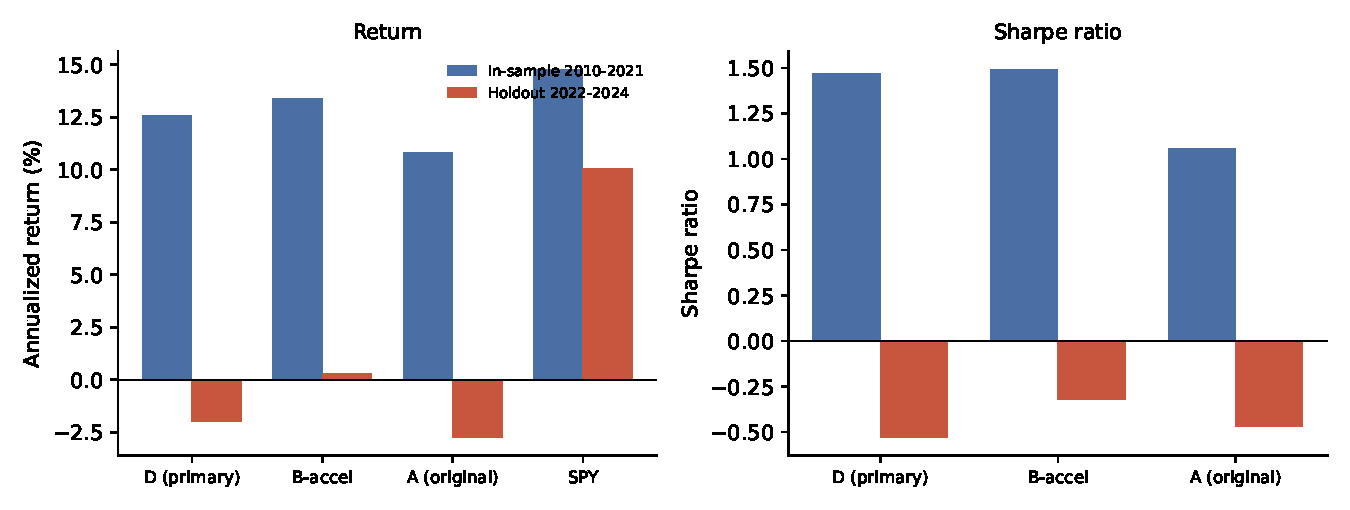
\includegraphics[width=\textwidth]{figures/fig_is_vs_oos.pdf}
\caption{In-sample (2010--2021) versus single-use holdout (2022--2024) for the three pre-registered arms and SPY (July runs). Generated by \texttt{figures/make\_figures.py} from the figures in Tables~\ref{tab:arms} and~\ref{tab:holdout}.}
\label{fig:isoos}
\end{figure}

Under the pre-registered reading, no arm was defensible out of sample. That is a valid outcome under the plan, and we recorded it as such.

\subsection{The central lesson: the one-shot test was spent on uncertified data}

Before looking at the reproduced results, we ran an independent eight-dimension data audit on the July database (its design is described in Section~\ref{sec:cert}). Its verdict was \emph{not fit} (NO APTA). Coverage, point-in-time correctness, accuracy against independent sources and internal consistency all scored D, the lowest grade. The finding most relevant to the holdout concerned coverage of \emph{current} fundamentals among point-in-time index members: 96.8\% in 2022 but 79.1\% in 2023 and 78.3\% in 2024. About 105 of 503 members had no current balance sheet, among them large names such as BRK.B, ABNB and AXON. The reason was mundane. Fundamentals for fiscal 2022 onwards came from a source without filing dates, and the bulk load of SEC EDGAR filings for 2023--2026 took place on 17 July, four days \emph{after} the holdout.

The engine-side preflight had passed the same window with zero blocking failures. It counted members that \emph{had} a fundamentals row. It did not check that the row was current, complete and point-in-time correct. The project therefore adopted a rule that it treats as non-negotiable: \emph{no run that counts is made on a database without an audit verdict of fit, or fit with reservations accepted in writing, and a frozen manifest} (row counts and content checksums per table). Under that rule the July holdout is invalid as a measurement. The window is still spent, because it has since been studied in depth and can never again serve as a clean test.

\paragraph{Did the data hole matter?} We fixed a decision rule before the rerun. The data effect would count as \emph{nothing} if the annual return moved by less than 1.5\,pp, \emph{some} if it moved by 1.5--4\,pp, and \emph{a lot} if it moved by at least 4\,pp with $t\ge 2$ and concentrated in the hole. We then reran the frozen arms on the corrected database as a diagnostic (Table~\ref{tab:holdout}). For arm~D the change was $+0.06$\,pp a year ($t=0.11$), split into $-0.63$\,pp in the control segment and $+0.74$\,pp in the hole segment. Portfolio overlap between the two runs (Jaccard) was 0.96 in the control segment and 0.88 in the hole. The data changed a few names in 2023--2024 and did not change the result. The verdict was \emph{nothing} for all three arms.

The lesson cuts both ways. The data defect did not cause the failure; the strategy failed on its own. Yet nobody could have known that \emph{ex ante}, and the only way to find out was a second look at a window that the protocol says should be seen once. Had the hole mattered, the project would have been left with an uninterpretable test and no clean window to replace it. A single-use holdout is a non-renewable resource, and certifying the data is a precondition for spending it, not a follow-up.

\paragraph{The failure recurred.} On 11 October 2026 the project spent a second single-use window, 1999--2008, which had been reserved for a pre-registered v2 model. The database had passed both the audit and the preflight. After the run, 91\% of the judge's evaluations turned out to be inconclusive for low data coverage. The judge's field coverage was 0.48, meaning only 13 of the 27 inputs it needs were present. The 1998--2008 load had left out 14 fields that the auxiliary source did contain (cash, operating income, capital expenditure, debt and others), so the portfolio held 1--3 stocks and 10--25\% equity throughout in all three arms. ``Neither the audit (which measures that a balance sheet is present, not complete) nor the preflight detected it'' (protocol log, 11 October). The run was declared invalid as a measurement. A second, explicitly labelled look followed after a data-only fix, which raised the judge's median field coverage from 0.48 to 0.93. The general point is that data checks must measure the completeness of \emph{the fields the model consumes}, at every decision date, not the presence of rows.

\subsection{Data certification}\label{sec:cert}

Between 8 and 26 October the database was rebuilt and certified by an audit agent with a fixed mandate. Data are judged only by data criteria (official filings, accounting identities, the market calendar), never by backtest results. Every correction is proposed with evidence, logged and approved by a human before it is written, with a backup taken first. The audit covers eight graded dimensions: coverage, point-in-time correctness, accuracy against independent sources (SEC \texttt{companyfacts}, Tiingo, yfinance; error rates with Wilson intervals), internal consistency, ticker identity (recycled tickers, dual classes), macro vintages (ALFRED), benchmark, and reproducibility (a manifest of row counts and content checksums). Its own test suite seeds known errors into a synthetic database and checks that they are detected.

The first round applied 231 of 258 proposed corrections. A full correction pass then logged items T-001 to T-202, and closed with four rounds of independent re-audit and correction. The number of high-severity findings fell from one critical and nine high in round~1 to one high in round~4. By the end every one of the 464{,}009 fundamental rows had a filing date. A cross-check against EDGAR of 1{,}307 company-year groups from fiscal 2022 onwards found 1{,}277 matching the original filing and 13 dated later than the filing (conservative). It flagged no automatic look-ahead. By hand, the audit found four spin-offs whose synthetic filing dates were too early (107 rows). They were corrected, with no effect on results because the firms entered the index later. The database was certified ``fit with reservations'' on 24 October 2026 for 1999--2008, 2009--2024 and 2025--2026, with no critical findings, and re-certified after each later correction. The accepted reservations are price splices, one-day spikes, small splits in as-traded prices and, before 2009, no structured SEC cross-check.

\subsection{Why the strategy failed: attribution of the gap}

The diagnosis was written under a stated rule: the 2022--2024 window is spent, so any ``what if'' is accounting decomposition, never a candidate change. It uses the diagnostic run of arm~D on the corrected database (9 October). Arm~D returned $-1.94\%$ a year against $+10.08\%$ for SPY in the engine's reported metrics, a gap of 12.0\,pp a year. On the grid between execution dates used for every decomposition below, D returned $-1.90\%$ against $+9.88\%$, a gap of 11.78\,pp a year.\footnote{\label{fn:grids}Three conventions appear in the project's records and in this paper. (i)~Engine metrics (\texttt{backtest\_metrics.json}, monthly decision grid): SPY 14.76\% a year in sample (2010--2021) and 10.08\% on the holdout; D $-1.94\%$ on the corrected database and $-2.00\%$ on the July database. Arm~A rebalances quarterly, so its SPY comparator is 8.26\% on the holdout and 14.92\% in sample. (ii)~Execution-to-execution grid of the diagnosis (periods between consecutive T+1 executions, annualised geometrically by days; 143 in-sample and 35 holdout periods): SPY 14.60\% and 9.88\%, D 12.38\% and $-1.90\%$. The two differ by the anchoring of periods and the annualisation convention, not by data. (iii)~Calendar-year figures (for example SPY $-18.6\%$ in 2022) are on the same execution grid, assigned by decision year. The cause shares quoted in the text (41\%, 28\%, 30\%) are each component divided by the 11.78\,pp grid gap: $4.85/11.78=41\%$, $3.26/11.78=28\%$, $3.52/11.78=30\%$, with bands and trend $0.15/11.78=1\%$; together they add to 100\%.} Figure~\ref{fig:cascade} and Table~\ref{tab:cascade} show the sequential cascade on the engine's grid.

\begin{figure}[t]
\centering
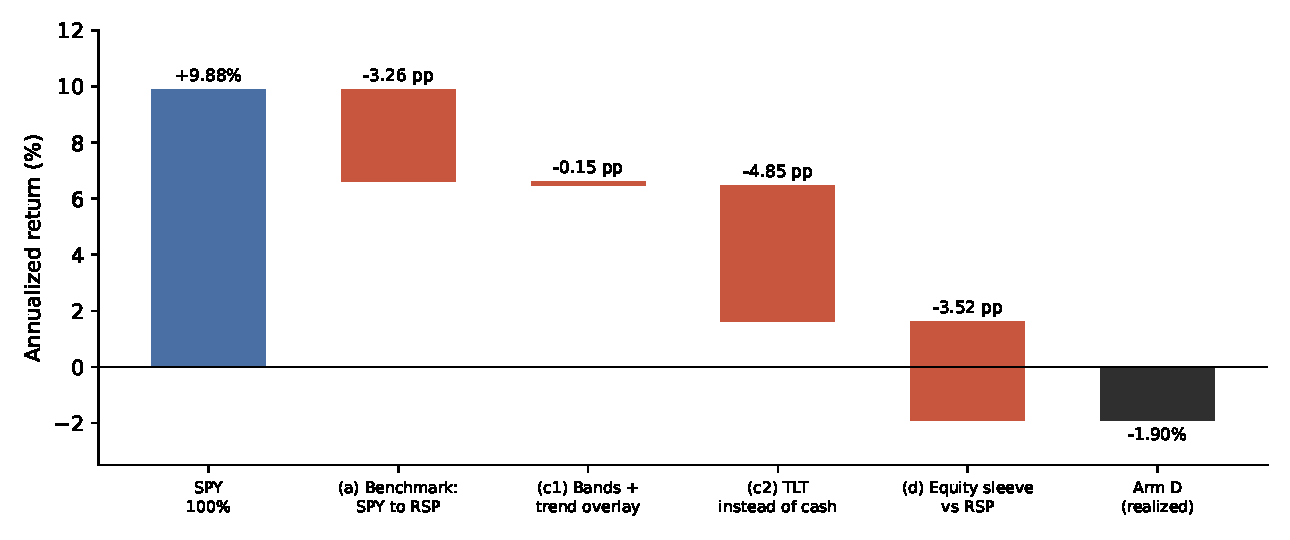
\includegraphics[width=0.92\textwidth]{figures/fig_gap_cascade.pdf}
\caption{Sequential attribution of arm~D's 2022--2024 gap to SPY, using D's realised weights, with the equal-weight S\&P~500 (RSP) as the index sleeve. Source: \texttt{research/diagnostico/DIAGNOSTICO\_2026-10-24.md}, \S2.}
\label{fig:cascade}
\end{figure}

\begin{table}[t]
\centering
\caption{Gap cascade, annualised, on the engine's execution-to-execution grid (conventions in footnote~\ref{fn:grids}). In sample, 2010--2021: 143 periods; holdout, 2022--2024: 35 periods.}
\label{tab:cascade}
\small
\begin{tabular}{lrrl}
\toprule
Step & In sample & Holdout & Holdout reading \\
\midrule
SPY 100\% & 14.60\% & 9.88\% & \\
RSP 100\% & 13.83\% & 6.62\% & (a) benchmark $-3.26$\,pp \\
D's weights, RSP sleeve, fixed income as cash & 9.25\% & 6.47\% & (c1) bands + trend $-0.15$\,pp \\
D's weights, RSP sleeve, fixed income as TLT & 11.72\% & 1.62\% & (c2) TLT vs.\ cash $-4.85$\,pp \\
D realised & 12.38\% & $-1.90\%$ & (d) sleeve vs.\ RSP $-3.52$\,pp \\
\midrule
Total gap to SPY & $-2.22$\,pp & $-11.78$\,pp & \\
\bottomrule
\end{tabular}
\end{table}

\paragraph{Duration risk (about 41\% of the gap).} The defensive sleeve was a 20-year Treasury fund. D held 26\% in TLT on average, and up to 49\% from May to October 2022. The same money in cash at the fed funds rate would have earned $+0.9$\,pp a year; in TLT it contributed $-3.4$\,pp a year. In 2022 alone, TLT explains $-12.2$\,pp of D's $-19.2\%$ NAV decline, while D's equity sleeve ($-10.7\%$) roughly matched RSP ($-11.7\%$). The regime made this worse. The yield-curve inversion flag, which shifted weight towards bonds, was active in 7 of 144 in-sample cycles (5\%) and in 30 of 36 holdout cycles (83\%). In sample, the few inversion episodes coincided with rising TLT, so the evidence rewarded the rule. The monthly stock--bond correlation (SPY--TLT) was $-0.43$ in 2010--2021 and $+0.68$ in 2022--2024, consistent with the macro drivers documented by \citet{CampbellPfluegerViceira2020}. In sample, TLT added $+2.5$\,pp a year over cash. The in-sample period rewarded exactly the design feature that sank the strategy out of sample.

\paragraph{Benchmark (about 28\%).} SPY minus RSP was 0.77\,pp a year in sample and 3.26\,pp a year on the holdout. In 2023 the whole SPY--RSP gap of about 12.5\,pp came from seven megacaps. D never held NVDA, MSFT, META, AMZN, GOOGL or TSLA. It held AAPL in 18 of 36 cycles. Against the engine's own equal-weight universe (7.26\% a year), the benchmark effect is 2.6\,pp, or 22\% of the gap, and the ranking of causes does not change. This is not a model error. It does mean that the pre-registered benchmark was poorly matched to a concentrated, roughly equal-weighted book.

\paragraph{Equity sleeve (about 30\%).} The sleeve lost 4.8\,pp a year to RSP, which is $-3.5$\,pp a year at portfolio level. Factor regressions of the implied monthly sleeve on Fama--French five factors, momentum and a low-variance factor (Table~\ref{tab:factors}) show stable loadings: beta 0.75--0.85, positive profitability and low-variance exposure, slightly anti-value. What changed was the environment. The low-variance premium realised $-7.5$\,pp a year in 2022--2024 ($-55.9$\,pp in 2023), against $+2.4$\,pp a year in sample. In-sample loadings times out-of-sample premia account for about $-1.9$\,pp a year at portfolio level. The residual, about $-1.0$\,pp a year, has $|t|<1$ in every specification. With 35 monthly observations, \emph{selection skill can be neither confirmed nor rejected}. The in-sample sleeve's FF7 alpha was $-0.1$\,pp a year ($t=-0.05$), so its in-sample ``edge'' was factor premia rather than selection.

\begin{table}[t]
\centering
\caption{Monthly factor regressions of the equity sleeve and of RSP ($t$-statistics in parentheses for the sleeve). Low-variance factor: bottom minus top quintile of the Kenneth French variance-sorted portfolios. Classical OLS standard errors; with $n=35$ the $t$-statistics are indicative only.}
\label{tab:factors}
\small
\begin{tabular}{lrrrr}
\toprule
Loading & Sleeve IS ($n=143$) & Sleeve OOS ($n=35$) & RSP IS & RSP OOS \\
\midrule
Mkt$-$RF & 0.85 (14.5) & 0.76 (7.7) & 0.95 & 0.86 \\
SMB & 0.26 (2.2) & 0.25 (1.7) & 0.20 & $-0.05$ \\
HML & $-0.16$ ($-1.6$) & $-0.21$ ($-1.4$) & 0.22 & 0.05 \\
RMW & 0.38 (2.7) & 0.21 (1.1) & 0.20 & $-0.19$ \\
Mom & 0.07 (1.1) & 0.11 (0.9) & $-0.02$ & $-0.21$ \\
LowVar & 0.19 (2.6) & 0.27 (2.6) & $-0.05$ & 0.09 \\
Alpha (pp/yr) & $-0.1$ ($-0.05$) & $-4.1$ ($-0.90$) & 0.3 & 0.1 \\
$R^2$ & 0.69 & 0.76 & 0.85 & 0.85 \\
\bottomrule
\end{tabular}
\end{table}

\paragraph{Brinson attribution.} A Brinson--Fachler decomposition \citep{BrinsonFachler1985,BrinsonHoodBeebower1986} of the reconstructed sleeve against the engine's equal-weight, point-in-time universe of 500 names (Table~\ref{tab:brinson}) splits the $-4.8$\,pp a year into allocation ($-2.2$), selection ($-2.5$) and interaction ($-0.1$). The allocation loss comes mostly from a 28\% weight in consumer staples, against 7\% in the universe, a sector that returned 0\% a year, and from holding no financials, energy or utilities. The selection loss is concentrated in 2023 and in logistics and services names (CHRW, EXPD, RHI) plus VRSN and AAPL. A single period beginning 3 January 2023 explains $-11.0$\,pp of the $-14.0$\,pp cumulative total. No effect has $|t|>1$. Sectors are the engine's SIC groupings, which misclassify several holdings; this moves the split between allocation and selection but not the total.

\begin{table}[t]
\centering
\caption{Brinson--Fachler attribution of the equity sleeve against the engine's equal-weight universe (pp, arithmetic sum of per-period effects).}
\label{tab:brinson}
\small
\begin{tabular}{lrrrr}
\toprule
 & Allocation & Selection & Interaction & Total \\
\midrule
2022 & $-1.90$ & $+4.21$ & $-1.57$ & $+0.74$ \\
2023 & $-1.04$ & $-7.95$ & $-3.13$ & $-12.11$ \\
2024 & $-3.50$ & $-3.55$ & $+4.45$ & $-2.60$ \\
\midrule
Per year & $-2.21$ & $-2.50$ & $-0.08$ & $-4.80$ \\
$t$ ($n=35$) & $-0.93$ & $-0.54$ & $-0.04$ & $-0.66$ \\
\bottomrule
\end{tabular}
\end{table}

\paragraph{Ruled out.} Trading costs were 0.45\,pp a year, the same as in sample. Execution lag was 1.5 days. The judge's behaviour (buy rate, Kelly fraction, probability of success) was unchanged between in sample and holdout. The tactical bands and trend overlay cost a net 0.15\,pp a year. Their slow 10-point re-entry cost about 2\,pp cumulatively in 2023.

\subsection{What the test window can and cannot conclude}

The pre-registered diagnosis classifies the outcome as a \emph{structural failure}. The causes are a duration bet embedded in the exposure rule, which met a rate shock, and a benchmark that became much harder to beat. Selection shows evidence neither for nor against. The window supports two conclusions. The in-sample Sharpe ratio of 1.47 was largely produced by falling rates and factor premia. The model also carried an untested duration bet: the in-sample period exercised the inversion rule in 5\% of cycles and always rewarded it. The window does \emph{not} support three others. It cannot tell whether stock selection works: three years, 14 names and $|t|<1$ cannot separate bad luck from a broken signal. It cannot tell whether the model would have worked ``with cash instead of TLT'' or ``with value''; choosing such a variant on this window is exactly what the protocol forbids. And it says nothing about the LLM layer, which was never evaluated. The only clean evidence that remains is forward. A paper-trading programme with pre-registered accounts starts on 1 November 2026 and will be evaluated after 9--10 months. Its evaluation rule was approved on 14 October 2026: no operational errors, maximum drawdown no worse than SPY's, and cumulative return no more than 3\,pp below an exposure-matched SPY. By the rule's own wording, passing shows that the system works as designed, not that it earns an edge.

\section{Lessons as a checklist}\label{sec:lessons}

Each item below is phrased as a check that a reviewer can answer yes or no, followed by the incident in this paper that motivates it.

\begin{enumerate}[leftmargin=*,itemsep=2pt]
\item \textbf{Certify the data before spending any single-use window.} Is there an independent audit verdict and a frozen manifest (counts and checksums) for the exact database used? \emph{July holdout; 1999--2008 window.}
\item \textbf{Measure completeness at the level of model inputs.} For each decision date, what fraction of the universe has every field the model consumes, current and point-in-time? Row presence is not enough. \emph{About 21\% of members without current fundamentals; only 13 of 27 judge fields present in 1999--2008.}
\item \textbf{Never bypass the preflight, and make it check what the model uses.} Is the skip flag disabled in runs that count? \emph{All research runs bypassed it until 30 June.}
\item \textbf{Treat cleaning code as model code.} Can any cleaning step use future information? \emph{The glitch guard deleted split stocks in all cycles.}
\item \textbf{Fix numeric acceptance thresholds in advance}, not only an ordering of metrics. \emph{The holdout reading criterion had none.}
\item \textbf{Choose the benchmark for the portfolio's construction}, and report a cap-weighted and an equal-weight benchmark side by side. \emph{SPY minus RSP: 0.8\,pp a year in sample, 3.3\,pp a year on the holdout.}
\item \textbf{Inventory implicit macro bets} (duration, inflation, stock--bond correlation) and count how often the in-sample period exercised each rule. \emph{Inversion rule active in 5\% of in-sample cycles versus 83\% of holdout cycles.}
\item \textbf{Count the trials and deflate the Sharpe ratio.} Report the number of configurations and validation looks, and compute the deflated Sharpe ratio or the probability of backtest overfitting \citep{BaileyLopezDePrado2014,BaileyEtAl2017PBO}. \emph{About 70 experiments and at least 12 validation looks; neither statistic was computed before the holdout.}
\item \textbf{Separate factor exposure from selection} before claiming skill. \emph{The in-sample sleeve's FF7 alpha was $-0.1$\,pp a year.}
\item \textbf{Version every output of a run that counts.} \emph{The original July outputs were lost; only an exact reproduction saved the record.}
\item \textbf{Keep LLMs out of historical decisions.} Treat any backtest of an LLM component over a period before its training cutoff as contaminated \citep{LopezLiraTangZhu2025,LiEtAl2025ProfitMirage}, and validate it forward only. \emph{The swarm is a narrative layer only.}
\item \textbf{Make the guard central and logged.} \emph{The guard was a per-clone local file; the July spend happened on another machine.}
\item \textbf{Do not let the reviewer share the developer's oracle.} \emph{Section~\ref{sec:toolkit}: 11 of 11 on the author's own cases, 5 of 12 on another author's; later 18 of 28 on a second reviewer's cases.}
\end{enumerate}

\section{The toolkit: \texttt{lockin-validate}}\label{sec:toolkit}

The figures in this section describe version 0.2.1 (28 October 2026); the use-case modules added in version 0.3.0 are described in Section~\ref{sec:usecases} and are taken only from the repository's README, changelog and documentation (check catalogue, validation evidence, alert policy, independent review and response, BYMA calendar notes, limitations).

\subsection{Scope and design principles}

\texttt{lockin-validate} reviews a strategy from the artefacts its author already has: prices, signals, trades, positions, costs, written rules and declared results. It does not run the author's model. It reconstructs positions, cash and NAV from the trades, runs data and strategy checks, reconciles them against the declared figures and writes a Markdown and JSON report. It is being consolidated from two internal prototypes built during the LockIn post-mortem, the \emph{LockIn Validate} prototype and the \texttt{revision} core, and is released as open source under the Apache 2.0 licence (version 0.2.1), at \url{https://github.com/joaquitodom/lockin-validate}. Five principles follow from the case study:

\begin{enumerate}[leftmargin=*,itemsep=2pt]
\item \textbf{Evidence-linked findings.} Every finding names the file, the rows, the dates and values involved, and the procedure that produced it. A finding without evidence is not reported.
\item \textbf{Never pass what was not verified.} Each finding has one status: \textsc{confirmed error}, \textsc{needs review}, \textsc{not executable} (with the reason) or \textsc{pass} within its stated scope. A check returns a pass only if it actually tested the property. A check whose inputs are missing, or whose test is only a hint, can never report a pass.
\item \textbf{Offline and deterministic.} The toolkit runs with no network and no remote AI, so a review is reproducible and client data never leave the machine. This is enforced in the test suite by blocking sockets.
\item \textbf{Read-only originals and logged transformations.} Inputs are hashed (SHA-256) into a manifest. Nothing is fixed silently. The report distinguishes diagnoses, proposed transformations and applied transformations, the last with before and after values.
\item \textbf{Independent oracle.} Expected results come from an implementation and a written specification that do not share code or conventions with the checks, and are complemented by synthetic cases with known answers and metamorphic tests \citep{BarrEtAl2015Oracle,SeguraEtAl2016Metamorphic}. Section~\ref{sec:crossreview} shows why.
\end{enumerate}

\subsection{Check catalogue mapped to failure modes}

Table~\ref{tab:checks} maps the checks inherited from 0.1.0 to the failure modes they target and to the incident or synthetic case that motivated each one. Table~\ref{tab:newchecks} covers the checks added in 0.2.x.

\begin{table}[t]
\centering
\caption{Checks inherited from \texttt{lockin-validate} 0.1.0 (28 of the 37 checks of 0.2.1, in five blocks: input, data, reconstruction, strategy, statistics; identifiers from \texttt{docs/CHECKS.md}). R-cases are the cross-review cases of Section~\ref{sec:crossreview}. ``Hint'' means the check can raise a review item but can never certify absence.}
\label{tab:checks}
\small
\begin{tabularx}{\textwidth}{>{\raggedright\arraybackslash}p{3.3cm}>{\raggedright\arraybackslash}X>{\raggedright\arraybackslash}p{3.7cm}}
\toprule
Failure mode & Check & Motivation \\
\midrule
Look-ahead via fundamentals & \texttt{pit\_fundamentals} (filing before period end, availability before filing, missing or implausible lags); \texttt{lookahead} (signal data available after the decision time) & PIT keying in LockIn; R04 \\
Undeclared look-ahead in a signal & \texttt{lookahead}: rank correlation between signal and subsequent return (hint, gross cases only) & R05 \\
Coverage holes / incomplete inputs & \texttt{coverage} (price coverage against the calendar), \texttt{essential\_fields} (empty key cells), \texttt{survivorship} (delisted members without prices) & July holdout; 1999--2008 window (partly; see text) \\
Duplicates, impossible dates, OHLC & \texttt{duplicates}, \texttt{dates} against a \emph{declared} calendar (NYSE, BYMA or none) & R11 \\
Corporate actions, glitches & \texttt{price\_jumps} (split-like, reverting spikes, unexplained), \texttt{corporate\_actions} (declared splits not applied) & Glitch-guard incident; R10 \\
Recycled tickers & \texttt{ticker\_identity} (with a security master) & LockIn identity issues \\
Wrong but coherent prices & \texttt{reference\_accuracy} (returns vs.\ an independent reference, Wilson interval) & Data audit, dimension 3 \\
Stale prices & \texttt{stale\_prices} & Prototype \\
Omitted or zero costs & \texttt{omitted\_costs} (commission and slippage separately; zero cost with turnover is a review item) & R01, R02, R08 \\
Wrong NAV base, shorts, leverage & \texttt{reconstruction} from initial cash; negative quantities or cash & H1 / R03, R06, R07 \\
Declared vs.\ reconstructed results & \texttt{results\_reconciliation}, \texttt{positions\_reconciliation}, \texttt{metrics} (convention vs.\ error) & R13 \\
Rules vs.\ implementation & \texttt{rules\_vs\_implementation}: re-executes rank, top-$N$, periodic rebalance and equal weight only & Process verification \\
Short records, smoothing & \texttt{sharpe\_significance} (Sharpe SE, PSR, MinTRL), \texttt{sharpe\_autocorrelation} (\citealt{Lo2002} factor, Ljung--Box) & Checklist item 8 \\
Selection bias & \texttt{trials\_declared}, \texttt{deflated\_sharpe}, \texttt{multiple\_testing} (Bonferroni, Holm, BHY haircut), \texttt{pbo} (CSCV) & About 70 LockIn experiments \\
LLM look-ahead & \texttt{llm\_lookahead\_risk}: risk score from declared design choices (always a review item) & Section~\ref{sec:related} \\
\bottomrule
\end{tabularx}
\end{table}

\paragraph{Checks added in 0.2.x.} Release 0.2.0 added nine checks in six families, each documented with its motivation in \texttt{docs/CHECKS.md}. Seven map to specific incidents of the case study. Table~\ref{tab:newchecks} maps them to the lessons of Section~\ref{sec:lessons}. Every one was written against \emph{lesson cases}: a planted positive and a clean negative per family, 16 cases in all, whose expected outcomes were committed before the checks existed. Two of the families (\texttt{liquidity\_participation} and \texttt{cost\_sensitivity}) do not answer a single LockIn incident. They make measurable an assumption that the LockIn backtests never tested, namely that every order fills at the close.

\begin{table}[t]
\centering
\caption{Checks added in \texttt{lockin-validate} 0.2.0 and revised in 0.2.1, mapped to the case-study lessons (checklist items of Section~\ref{sec:lessons}). Descriptions condensed from \texttt{docs/CHECKS.md}.}
\label{tab:newchecks}
\small
\begin{tabularx}{\textwidth}{>{\raggedright\arraybackslash}p{3.4cm}>{\raggedright\arraybackslash}X>{\raggedright\arraybackslash}p{3.3cm}}
\toprule
Check & What it checks & Case-study lesson \\
\midrule
\texttt{coverage\_drift} & Per input field and period, the share of universe members with a valid value; review when coverage falls at least 10\,pp below the median of earlier periods. Periods without any row count as 0\% up to the last period the strategy uses. & July holdout ($\approx$21\% without fundamentals); items 1--2 \\
\texttt{input\_sufficiency} & For every scored row, how many declared \texttt{required\_inputs} have a value, as of the decision and no older than 400 days; confirmed error only when a declared minimum is broken unambiguously. & 1999--2008 window (13 of 27 inputs); item 2 \\
\texttt{protocol\_integrity} & A run log against a declared protocol: runs touching a reserved window, more than one configuration on the test window, ``reproductions'' of configurations never tested there, development after the test look, validation looks counted as trials. & Spent windows; items 1, 8, 12 \\
\texttt{benchmark\_fit} & Beta, tracking error and information ratio against the declared benchmark and the equal-weight universe; gap split into benchmark-choice and selection effects; review when the benchmark's construction differs from the strategy's. & SPY vs.\ equal weight ($\approx$3\,pp a year); item 6 \\
\texttt{dividend\_} \texttt{corporate\_actions} & Adjusted vs.\ as-traded ratio on declared ex-dates: dividends not applied, wrong step sizes, prices frozen after an ex-date, total return equal to price return. & Frozen prices in paper trading; items 3--4 \\
\texttt{liquidity\_} \texttt{participation}, \texttt{cost\_sensitivity} & Orders vs.\ average and same-day volume (per ticker-day); break-even cost and results at 1$\times$, 2$\times$ and 3$\times$ declared costs. & Fill-at-close assumption (no single incident) \\
\texttt{stability\_and\_} \texttt{concentration}, \texttt{conditional\_rule\_} \texttt{activation} & Subperiod, name and day concentration of the result; share of periods each declared conditional rule is active in and out of sample (review below 10\% in, above 50\% out). & Inversion rule: 5\% vs.\ 83\% of periods; item 7 \\
\bottomrule
\end{tabularx}
\end{table}

\paragraph{What is and is not covered now.} The central failure of Section~\ref{sec:results} is now detected in synthetic reproductions. The independent reviewer's LockIn-like case (V28) plants a fall in fundamentals coverage from 97\% to 79\% in 2022--2024, on a package whose point-in-time and protocol checks pass. \texttt{coverage\_drift} flags it (``97\% to 79\%''), and the corresponding lesson case (L01, 97\% to 80\%) is also caught. On 0.2.0, \texttt{input\_sufficiency} met the stretch expectation of V28 for the wrong reason: it fired on warm-up months, not on the test years, because as-of fundamentals never expired. Release 0.2.1 expires them after 400 days, and the test years are now flagged. A reserved window scored with half of its declared inputs (lesson L03) is a confirmed error. Three limits remain. First, \texttt{input\_sufficiency} judges only the inputs the owner declares in \texttt{required\_inputs}, so the 1999--2008 failure is caught only if the 27 judge inputs are declared. Second, without a declared universe the members are the tickers present in the table, so a genuinely shrinking universe reads as drift, and members absent from every input are invisible. Third, the checks see only what is delivered. They cannot say which value is right, and \texttt{protocol\_integrity} cannot see runs that were never logged. The LLM check remains a risk score from declarations: memorisation is never tested, so it never passes.

\subsection{Cross-review methodology and results}\label{sec:crossreview}

We used the same procedure in two rounds. A reviewer that is not the package's author writes its own cases with a seeded generator that does not import the package. It fixes the expected outcomes and commits them \emph{before} the tool is run, and none of its files are edited afterwards. The authors may change only the code, never the reviewer's expectations. In both rounds the reviewer was an AI agent in a separate role, not a human; Section~\ref{sec:limits} discusses what that implies.

\paragraph{Round 1 (internal core, 21 October).} The core's own battery gave 11 of 11; the reviewer's 12 cases gave 5 of 12. The worst defect was a textbook correlated failure. The return was measured from the NAV of the first day, \emph{after} the first trades, so first-day costs disappeared from return and Sharpe ratio. With a 0.85\% commission the tool overstated the return by 0.89\,pp and accused an honest client, whose final NAV matched to the cent. The package, its ``independent'' verifier, a hand-computed spreadsheet and the case simulator all shared that convention \citep{KnightLeveson1986}. Three checks reported ``correct'' without having verified anything: unrecognised result keys, a signal equal to the future return, and zero costs with 100\% turnover. BYMA trading days were flagged as errors under a default NYSE calendar. After code-only fixes the core matched 12 of 12 with 63 tests. These 12 cases are now the adversarial part of the release battery. They were ported with every expected outcome unchanged, and a value-by-value comparison with the originals found 0 mismatches.

\paragraph{Round 2 (release 0.2.0, 28 October).} The reviewer wrote 28 pre-registered cases: 13 subtle planted problems or verification gaps, 12 clean packages built to tempt false positives, 2 end-to-end packages and 1 LockIn-like holdout. On 0.2.0 the battery verdict was 18 of 28. Firm detections were 15 of 21, 9 of 12 clean cases were correct on their target check, and there were 4 false positives. The six misses shared one pattern: a check returned a pass on a package it could not, or did not, verify. Examples are \texttt{coverage\_drift} passing when a vendor stopped delivering all fundamentals, a dividend check passing with zero events checked, and a declared conditional rule silently dropped. Two confirmed errors rested on ambiguous evidence, one from the letter case of input names and one from a test look labelled ``holdout''. Release 0.2.1 fixed these in code. The result was 27 of 28, obtained against the same cases that guided the fixes, with firm detections 21 of 21, clean cases 12 of 12 and 1 false positive. The remaining failure, V18, is a defect of the reviewer's generator: a sell before any buy in a shared counter, which the reviewer documented. The tool's confirmed error there is correct for the trades delivered, and the case's target check passes, so we left the case failing rather than suppress a true finding.

\paragraph{Alert noise: mostly relabelling.} Release 0.1.0 raised 40 unexpected review items across its 36 cases. Release 0.2.0 introduced an \textsc{info} status with three written rules: the same evidence is judged elsewhere, the note describes strength of evidence below a documented threshold, or there is nothing declared to contradict. It also reclassified every one of the 40. The reviewer disputed the bookkeeping, and the project's alert policy now states the result plainly: the reduction from 40 to 3 is ``mostly relabelling, not a change of the tool.'' Of the 40, 20 are now expected by their cases after the output was seen (post hoc), 16 are \textsc{info} notes, 1 was a bug and 3 expectations were withdrawn. Since 0.2.1 the battery reports pre-registered detections and post-hoc expectations on separate lines and never sums them. The reviewer also noted that the threshold behind most \textsc{info} downgrades (\texttt{significance\_review\_ratio} $=2$) was chosen with the battery in view. Its sensitivity is now disclosed: at ratios 1, 1.5, 2, 3 and 5, the battery's below-threshold Sharpe cases produce 23, 19, 9, 6 and 4 review items. The battery is not cited as support for the value 2. A second change, which narrowed the single-lag band of the autocorrelation-adjusted Sharpe test from 1.96 to 2.576, was checked by a seeded Monte Carlo (2{,}000 draws, $T=250$ and $1{,}250$). The full review rule had an empirical size of 0.017--0.024 with the old band and 0.010--0.015 with the new one, so it was not oversized, and the change is recorded as a refinement rather than a bug fix.

\paragraph{Release evidence (0.2.1).} The catalogue has 37 checks: 28 from 0.1.0 and 9 new. The test suite gives 187 passed and 1 skipped; the skipped test builds the optional MCP server and passes with that extra installed. The linter is clean. GitHub Actions continuous integration (\texttt{ci.yml}) runs lint, tests, the benchmark battery and a case-reproducibility check on Ubuntu and Windows with Python 3.10, 3.11 and 3.12, and passed on 0.2.1. The team's own battery has 52 synthetic cases: 11 core, the 12 round-1 adversarial cases, 7 statistical, 6 data and 16 lesson cases. All 52 produce all their expected outcomes. Pre-registered detections are 52 of 52, reported separately from the 20 of 20 post-hoc expectations, with 0 false positives and 6 unexpected review items. Independent verification includes a hand-computed case reproduced by the package, by an oracle that does not import it and by empyrical-reloaded, and agreement to $10^{-9}$ on NAV, cash and metrics across six core cases. The deflated Sharpe ratio reproduces the numerical example of \citet{BaileyLopezDePrado2014}. There are also metamorphic tests and a socket-blocked offline run.

\paragraph{A calendar finding.} Building a sourced BYMA (Buenos Aires) holiday calendar for 2015--2026 turned up a small finding of its own. The packaged file lists 206 closed days: 159 verified, 35 partially verified and 12 not verified. BYMA treats ``d\'ias no laborables'' (non-working days that are not holidays) inconsistently over time. It closed on the 2018--2019 tourism days and on 2 May and 15 August 2025, but traded on 21 November 2025, and Bank Employees' Day closed the market in some years and not in others. The widely used \texttt{exchange\_calendars} XBUE calendar (version 4.13.2) disagrees with the file on 49 days, 44 of them from 2020 onwards. An independent sample of 10 dates found no contradictions, but 5 of the 10 rest on secondary evidence only.

\section{Use-case modules (version 0.3.0)}\label{sec:usecases}

The failures reported in Sections~\ref{sec:results} and~\ref{sec:lessons} concern a trading strategy, and the core of \texttt{lockin-validate} reviews exactly that. The same questions arise for other kinds of financial model: whether a score predicts anything before it becomes a strategy, whether a machine-learning classifier was evaluated out of sample, whether a published Value at Risk was honoured, whether a forecast beats a naive benchmark, whether a set of target weights respects its mandate, and whether a live record resembles the backtest that justified it. Version 0.3.0 (6 November 2026) adds six \emph{use-case modules} for these questions. The core checks are unchanged. The figures in this section come from the repository's changelog, the per-module documentation (\texttt{docs/usecases/}), the module development guide and the two review reports with their responses. The modules are review aids. They are not a certification, a statement of regulatory compliance or a substitute for model-risk governance, and no statement here concerns profitability.

\subsection{Registry, activation and status contract}

A module is one file that declares its input tables, column aliases, requirements, catalogue entries, references, numeric conventions and review profiles in a single specification, and registers it at import time. Registration merges these declarations into the package-wide tables, so no core file is edited when a module is added. A module runs automatically when one of its detection files is in the input folder (for example \texttt{signals.csv}, \texttt{var\_forecasts.csv}, \texttt{forecasts.csv}, \texttt{weights.csv}, \texttt{live\_returns.csv}). It can also be forced on the command line, in which case every check whose tables are absent reports \textsc{not executable} with the name of the missing input, rather than silently disappearing.

The status contract of Section~\ref{sec:toolkit} carries over without relaxation. \textsc{Confirmed error} is allowed only when the input itself proves the error (a target date before its forecast origin, a test sample inside the training window, weights summing to 1.3 under a declared no-leverage rule). A statistic that crosses a documented threshold gives \textsc{needs review}. A missing or too short input gives \textsc{not executable}. \textsc{Pass} is reserved for a property that was verified on enough data and is never returned on an empty or trivial input. Every finding carries evidence rows, a sentence describing the procedure and an action, and every threshold is a named convention with a default that the user's rules file can override. Modules use only \texttt{numpy} and \texttt{pandas} and implement their test statistics directly, which keeps the offline and deterministic property. Each module ships with generated cases whose expected outcomes are written from the planted problem before the tool is run, and the development guide requires at least a clean case, one case per check, an adversarial case in each direction (looks fine but hides the problem; looks wrong but is legitimate) and an insufficient-data case. In total the modules add 35 checks (72 in the package) and 57 cases (109 in the battery).

\subsection{The six modules}

Table~\ref{tab:modules} summarises the modules. The paragraphs below give, for each, the question it answers, its audience and inputs, and the statistical tests behind its checks.

\begin{table}[t]
\centering
\caption{The six use-case modules of version 0.3.0. ``Detect file'' is the input whose presence activates the module. Case counts are the module's own synthetic cases.}
\label{tab:modules}
\small
\begin{tabularx}{\textwidth}{>{\raggedright\arraybackslash}p{1.6cm}>{\raggedright\arraybackslash}p{3.6cm}>{\raggedright\arraybackslash}X>{\raggedright\arraybackslash}p{1.5cm}}
\toprule
Module & Detect file & Question & Checks / cases \\
\midrule
\texttt{signals} & \texttt{signals.csv} (with prices) & Does the score rank forward returns, how fast does it decay, what turnover does it imply? & 5 / 8 \\
\texttt{ml} & \texttt{ml\_samples.csv}, \texttt{ml\_predictions.csv} & Was the model evaluated out of sample, is it calibrated and stable? & 6 / 12 \\
\texttt{risk} & \texttt{var\_forecasts.csv} & Do realised exceptions match the promised VaR and ES coverage? & 6 / 8 \\
\texttt{forecast} & \texttt{forecasts.csv} & Were forecasts made before the fact, do they beat a naive benchmark? & 6 / 8 \\
\texttt{portfolio} & \texttt{weights.csv} & Do the weights respect declared constraints and add value over $1/N$? & 6 / 11 \\
\texttt{live} & \texttt{live\_returns.csv} & Does the live record behave like its shadow backtest? & 6 / 10 \\
\bottomrule
\end{tabularx}
\end{table}

\paragraph{\texttt{signals}: alpha signal research.} The module is for researchers who hold a cross-sectional (or single-asset) score and want to know whether it predicts returns before it becomes a strategy. Inputs are decision dates, tickers and signal values, plus prices. A decision dated $t$ enters at the close of the first session at or after $t$ plus a declared lag (default one session) and is evaluated over a set of horizons, so that no same-close information enters the forward return. The checks cover forward-return alignment, the per-date Spearman rank information coefficient (IC) with a \citet{NeweyWest1987} $t$-statistic whose lag length follows the overlap between horizon and decision spacing, the quantile spread and its monotonicity, rank autocorrelation with top-bucket turnover and half-life, and a hint of look-ahead from the IC with the contemporaneous return. The $t=3$ hurdle of \citet{HarveyLiuZhu2016} is quoted as context and is not a review threshold. A predictive signal is a judgement, so the IC check never returns a pass. When the cross-section is too thin on every date, the IC is computed through time within each ticker, with a caution that this is noisier.

\paragraph{\texttt{ml}: supervised model validation.} The audience is the data scientist and the model-risk team who must judge the evaluation protocol of a model that is already trained. The module never refits it. Inputs are a sample table (timestamp, split, and the time at which each label becomes known), the delivered predictions, and optionally feature metadata and values. Six checks cover (i) split leakage: shared sample identifiers, test timestamps inside the training range, training labels that end after the first test timestamp (no purging), embargo gaps and, under a declared purged $K$-fold, the same conditions inside each fold, following the purging and embargo logic of \citet{LopezDePrado2018}; (ii) the train, validation and test gap in AUC (with the standard error of \citealt{HanleyMcNeil1982}) or in $R^2$ for regressions; (iii) probability calibration through expected calibration error, the Brier score and its Murphy decomposition, and the Hosmer--Lemeshow statistic \citep{HosmerLemeshow1980}; (iv) population stability (PSI) and a label-shift test; (v) target leakage in features; and (vi) the number of models scored on the test split against the declared number of trials, in the spirit of \citet{BaileyLopezDePrado2014}. A population stability index above its high threshold raises a review item at high priority but never a confirmed error, because it is a statistic and not a proof.

\paragraph{\texttt{risk}: VaR and ES backtesting.} The audience is risk managers and validation units that publish a Value at Risk. The input is one table with the date, the realised P\&L and one or more VaR (and optionally ES) forecasts made before the day. The module does not estimate a VaR or judge methodology. Six checks cover input coherence (sign convention, ordered quantiles, ES at least VaR), unconditional coverage with the proportion-of-failures test of \citet{Kupiec1995}, independence and conditional coverage with the Markov tests of \citet{Christoffersen1998}, the Basel traffic-light zones \citep{Basel1996}, an Expected Shortfall test of \citet{AcerbiSzekely2014}, and a chi-square homogeneity test of exception rates across sub-periods (whether the model reacts to volatility). The coverage decision uses the exact binomial acceptance region and prints the asymptotic likelihood ratio as context, since the asymptotic test over-rejects when about three exceptions are expected (for example, zero exceptions in 260 days at 99\%: asymptotic $p=0.022$, exact $P(X=0)=0.073$). Too few exceptions are reported as a review item distinct from too many, because an over-conservative model costs capital and hides whether it responds to stress.

\paragraph{\texttt{forecast}: point forecasts.} The audience is economists, strategists, treasury and planning teams and time-series modellers. The input is a table of forecasts with origin date, target date, forecast and realised value, and optionally model, series, horizon, release date of the actual and a benchmark. The checks cover origin integrity (a target before its origin, actuals not yet published at the origin, exact duplicates), a comparison with a naive benchmark through the \citet{DieboldMariano1995} test with the small-sample correction of \citet{HarveyLeybourneNewbold1997}, bias through the joint Wald test of the \citet{MincerZarnowitz1969} regression, direction through the \citet{PesaranTimmermann1992} test, error dynamics (Ljung--Box and a multi-step variant, since $h$-step errors are autocorrelated by construction), and an expected-maximum selection check when several models are compared. Horizons are counted in observation steps of the series, not in calendar days.

\paragraph{\texttt{portfolio}: target weights.} The audience is portfolio managers, allocators and compliance teams who receive a table of target weights (an optimiser output, a model portfolio, an index tracker) and must decide whether to trust it. Optional inputs are prices, positions, benchmark weights and returns, and a block of declared constraints. The checks cover whether declared constraints hold on every date (long-only, weight bounds, leverage, net exposure, group limits, turnover); concentration by HHI, effective number of names, top-five weight and group weights; turnover net of drift and the rebalance schedule; weights against positions times prices; the Sharpe difference against $1/N$ \citep{DeMiguelGarlappiUppal2009}, with the test of \citet{JobsonKorkie1981} in the form corrected by \citet{Memmel2003}; and active share against a benchmark \citep{CremersPetajisto2009} as a closet-indexing indicator.

\paragraph{\texttt{live}: live track record.} The audience is managers who went live or began paper trading, allocators doing due diligence and risk committees. The question is not whether the backtest was honest but whether the strategy in production behaves like its simulation. Inputs are the live return or NAV series, the backtest series (ideally a shadow backtest run over the live dates), and optionally live and model trades and declared metrics. The checks cover period integrity against the declared start, live against shadow backtest (tracking error, mean-difference test with a HAC variance, Sharpe difference and probabilistic Sharpe ratio), performance decay against an expected out-of-sample haircut, structural break (a CUSUM scheme in the tradition of \citealt{Page1954} and a mean-shift test), execution quality (slippage, fill ratio, overrides) and declared against realised metrics. The expected haircut of 0.5 on the Sharpe ratio is a published average and not a property of any strategy, and the documentation says so.

\subsection{Validation evidence for the modules}

\paragraph{Own battery.} The 57 module cases (signals 8, ml 12, risk 8, forecast 8, portfolio 11, live 10) are written by the module's author from the planted problem before the first run. Together with the 52 earlier cases the battery has 109 cases. At release all 109 produce their expected outcomes, with 159 of 159 pre-registered detections and no false positive. As with the 52-case battery, this is a regression result on cases written by the same team that wrote the code, and it does not estimate accuracy on unseen problems (Section~\ref{sec:limits}).

\paragraph{Two pre-registered adversarial reviews.} We repeated the procedure of Section~\ref{sec:crossreview} for the modules. Reviewer A (signals, ml, forecast) wrote 18 cases and reviewer B (risk, portfolio, live) wrote 33, each with a seeded generator that does not import the package and with expected outcomes fixed before the first run. The authors changed only code, never the reviewers' files, and documented each disagreement. Reviewer A's score rose from 13 to 17 of 18 cases (pre-registered detections 24 of 28 before, 28 of 28 after). Reviewer B's score rose from 29 to 30 of 33. As in round 2 of Section~\ref{sec:crossreview}, the post-fix scores were obtained after fixing the code against the same cases and therefore measure responsiveness to review, not accuracy on unseen cases. Both reviewers were AI agents in a separate role.

The defects fall into a small number of classes, several of which echo the incidents of the case study.
\begin{itemize}[leftmargin=*,itemsep=2pt]
\item \emph{Tie handling.} Tied signal values were split into buckets by file order, so a graded score with no skill produced a significant quantile spread (+54.6\,bp, $t=4.09$) from a ticker fixed effect. Tied values now share a bucket by average rank, and a constant signal makes turnover and spread \textsc{not executable}.
\item \emph{Missing and non-finite values.} Rows with a blank probability entered the AUC as the top score, so different checks used different sample sizes. A missing NAV merged two returns into one two-period return and doubled the apparent tracking error (1.36\% against 0.654\% after the fix). Blank probabilities are now dropped before every metric and disclosed, and a missing NAV yields two missing returns.
\item \emph{Silent passes in degenerate cases.} An undefined test AUC (no positives) was reported as a gap ``within the threshold'', and calibration passed when the observed base rate was exactly zero against a mean predicted probability of 0.049. These are the same defect as the checks that passed without verifying anything in Section~\ref{sec:crossreview}. An undefined statistic is now \textsc{not executable} or a review item, never a pass.
\item \emph{Calendar versus step horizons.} Weekend gaps in business-day forecasts were read as multi-day horizons, splitting a one-step series into a spurious three-step group with the wrong Newey--West lags. Horizons are now steps in the series' own target dates. A related fix makes the gap rule in \texttt{live} relative to the native frequency, because monthly records were flagged as gaps.
\item \emph{Drift versus trading.} A constant target printed on a schedule produced a false confirmed error for off-schedule trading, because weights drift with prices even when nothing is traded. The check now judges changes in the delivered target weights. A residual limit remains: a system that really trades back to target each month and exports the same target row is indistinguishable from a constant table, and the report says so.
\item \emph{Decision inconsistent with the printed evidence.} The Kupiec message used the asymptotic test while printing the exact acceptance region, so the two could disagree. The exact region now decides.
\item \emph{Applicability and units.} Short-only and market-neutral books were compared with long-only $1/N$; they now receive \textsc{not executable} with the reason. Returns delivered in percent units are flagged. Exact duplicate forecasts passed a minimum-sample gate and are now dropped and disclosed.
\end{itemize}

\paragraph{Monte Carlo checks of two decision rules.} Two rules were examined by simulation (seeded, 2{,}000 replications per cell). In \texttt{forecast}, the former bias rule flagged a forecast if either the Wald test or $|t|>2$ rejected; under a true model its false-alarm rate was 12.5\% at $n=30$ (10.0\% at 60, 7.8\% at 300). The rule now uses the joint Wald test alone, whose rate is 10.6\%, 7.9\% and 5.9\% at those sample sizes. In \texttt{live}, a one-sided 5\% test that the live mean return is below zero, using an asymptotic HAC variance, had size 8.6\% at $n=30$ with independent returns. With a small-sample variance factor, a $t(n-1)$ critical value and, below 60 periods, a further requirement that the iid $t$-statistic also reject, size is 5.0\% at $n=30$. Under an AR(1) process with coefficient 0.3, size at $n=30$ falls from 10.2\% to 7.8\%, and at $n=24$ from 10.8\% to 8.7\%. Tightening further would cost power on true alerts.

\paragraph{Disputed cases and remaining failures.} The reviewers' batteries still show four failed cases. One in the first review (a signals case) fails solely because the core completeness check raises a confirmed error for 92 blank signal cells, which we regard as correct behaviour. In the second review, one case encodes the reviewer's own error (an ES set at 70\% of its true value falls below the VaR, so the coherence error is right). In another, the reviewer's expectation of a review item for zero exceptions in 260 days at 99\% rests on the asymptotic $p$-value that the first fix showed to contradict the printed region. In the third, the module follows the documented conditional-coverage rule while the reviewer expected independence alone; we corrected the wording and kept the status. We record these as disagreements and did not edit the reviewers' expectations.

\subsection{Limitations specific to the modules}

The modules inherit the limitations of Section~\ref{sec:limits}. In addition: (i) the evidence is synthetic cases and two AI-agent reviews, with no human reviewer and no application to a third party's real artefacts; (ii) the small-sample corrections reduce but do not remove size distortion, and under autocorrelation the \texttt{live} test remains above its nominal level at small $n$, as does the Wald bias test in \texttt{forecast}; (iii) several tests have low power at the minimum sample sizes (Kupiec below about 250 days, a Markov test with fewer than five exceptions), and a pass says only that the test did not reject; (iv) inputs are taken as delivered, so live returns are not checked against broker statements and forecasts are not checked against vendor vintages unless release dates are supplied; (v) thresholds and the 0.5 Sharpe haircut are conventions, not properties of a strategy; (vi) the Basel traffic light and the ES test are the published procedures applied to the user's table, and a finding is not a supervisory classification; and (vii) the modules check the evaluation and the delivered numbers, not whether the underlying model or mandate is appropriate.

\section{Limitations and threats to validity}\label{sec:limits}

\paragraph{Self-assessment.} We designed the strategy, ran the holdout, audited the data, wrote the diagnosis and built the toolkit. Nothing here meets the ``effective challenge'' standard of \citet{SR117}. Much of the audit, diagnosis and toolkit work was carried out by AI coding agents under our supervision. The cross-review was one agent reviewing another, which shares training biases. We report it as \emph{AI-assisted review verified against known-answer cases}, not as independent validation.

\paragraph{Synthetic cases and reviewers.} The toolkit's figures come from synthetic cases, which say little about detection rates on real artefacts. Except for the 12 round-1 adversarial cases, the 52-case battery was written by the same team that wrote the code, so 52 of 52 is a regression result, not an independent accuracy estimate. The 28 round-2 cases are independent of the code but not of its documentation. Both reviewers were AI agents in a separate role, which is not the independent human challenge of \citet{SR117}. The round-2 score of 27 of 28 was obtained after fixing the code against those very cases, so it measures responsiveness to review rather than accuracy on unseen problems. Some thresholds (for example \texttt{significance\_review\_ratio}) were chosen with the battery in view; their sensitivity is disclosed, not justified by it. The look-ahead hint catches only gross leaks. Rule re-execution is limited to rank, top-$N$, periodic rebalancing and equal weight. Several BYMA days rest on secondary evidence. Limitations specific to the use-case modules are in Section~\ref{sec:usecases}.

\paragraph{Data.} Free data impose a survivorship floor of about a dozen delisted names that we could not cover. Before 2009 there is no structured SEC cross-check. The certified database still carries accepted reservations. The diagnostic rerun in Table~\ref{tab:holdout} ran on the corrected database of 9 October, which later rounds of correction changed again. We did not rerun it, because the window is spent and the earlier verdict was already \emph{nothing}.

\paragraph{Statistics.} Out-of-sample inference rests on 35 monthly periods. Regressions use classical standard errors, and every selection effect has $|t|<1$. The equity sleeve is implied from NAV, bond and cash weights. The cascade closes to 0.01\,pp only because it is an accounting identity, not because the sleeve is measured that precisely. The Brinson split depends on the SIC taxonomy. We computed no rank information coefficient for the score, and no formal deflated Sharpe ratio or probability of backtest overfitting.

\paragraph{Protocol leakage.} The test window was touched three times before the valid run, as declared. Validation was reused heavily. The 2022--2026 period has since been examined for several defensive rules. The second single-use window (1999--2008) was looked at twice, as declared. Forward paper trading is therefore the only clean evidence left.

\paragraph{Generality.} This is one strategy family, one market and one three-year regime that was unusually hostile to both duration and equal-weight portfolios. We offer the episode as a worked example of how a protocol fails, not as an estimate of how often it does.

\section{Conclusion}\label{sec:conclusion}

A pre-registered, single-use holdout did what it was designed to do: it stopped us from shipping a model whose in-sample Sharpe ratio of 1.47 came from falling rates and factor premia. It also showed that a protocol is only as good as the data it runs on. We spent the one shot before certifying the data, and later repeated the mistake in another window. Luck spared us in the first case, because the data defect turned out not to matter. Checks that measured the presence of rows rather than the completeness of the model's inputs failed us in the second. The attribution assigns the failure to an untested duration bet and a mismatched benchmark, and finds no evidence either way on stock selection. We turned these lessons into a checklist and into \texttt{lockin-validate}, whose own first cross-review provided one more lesson: a verifier that shares the developer's conventions will agree with the developer's mistakes. The same discipline now extends, in version 0.3.0, to six other uses of validation (signals, supervised models, VaR and ES, forecasts, portfolio weights and live records). There two further reviews found defects of familiar kinds, such as silent passes on degenerate input, ties, missing values and mismatched horizons, and the residual size distortion and disputed cases remain disclosed. The remaining open question, whether the strategy has any edge, will be answered forward or not at all.

\section*{Data and code availability}
Figures are generated by \texttt{figures/make\_figures.py} from numbers transcribed from the cited repository documents; no price or vendor data are redistributed. \texttt{lockin-validate} is available at \url{https://github.com/joaquitodom/lockin-validate} under the Apache 2.0 licence, together with its synthetic benchmark cases and their generators. The LockIn diagnostic scripts are not released, because they depend on licensed vendor data.

\section*{Acknowledgements}
This paper extends the first author's MSc thesis at the Universidade de Vigo (tutor: Francisco Rodr\'iguez de Prado). AI coding assistants were used for data auditing, diagnostics, toolkit development and drafting, under the authors' supervision; all numbers were checked against the project's records. Any errors are ours.

\bibliographystyle{plainnat}
\bibliography{refs}

\appendix
\section{Timeline of the validation record}\label{app:timeline}
\small
\begin{tabularx}{\textwidth}{lX}
\toprule
Date (2026) & Event (source: \texttt{.planning/PROTOCOL-LOG.md}, \texttt{gestion/estado.json}) \\
\midrule
10 Jun & Out-of-protocol preliminary run on the test window; discarded and declared. \\
11--13 Jun & Train and validation looks; measurement fixes reveal zero equity purchases under calibrated base rates; calibration embargo. \\
30 Jun & Preflight found to be bypassed in all runs; glitch-guard look-ahead fixed; survivorship floor accepted. \\
3--4 Jul & Configurations frozen; holdout spend plan and comparative addendum (arms D, B-accel, A). \\
13 Jul & Holdout spent (commit \texttt{05cd144}); no arm defensible out of sample. \\
17 Jul & EDGAR 2023--2026 fundamentals loaded, after the holdout. \\
8 Oct & Exact reproduction of the three arms; audit of the July database: not fit (current fundamentals 79.1\% in 2023, 78.3\% in 2024). \\
9 Oct & 231 corrections applied; diagnostic reruns on corrected database (data effect: \emph{nothing}). \\
11 Oct & Second single-use window (1999--2008) spent; invalid (91\% inconclusive from missing fields); declared second look after data-only fix. \\
19--26 Oct & Full database correction (T-001 to T-202), four independent re-audit rounds; certified 24 Oct, re-certified 25--26 Oct. \\
21 Oct & Toolkit core cross-review: 5 of 12, then 12 of 12 after code-only fixes (63 tests). \\
24 Oct & Diagnosis and Brinson attribution completed. \\
1 Nov & Pre-registered forward paper trading begins (scheduled). \\
\bottomrule
\end{tabularx}

\end{document}
